\chapter{Практические задания}

\section{Задание 1}

На рисунках \ref{1_1}~--~\ref{1_6} представлены списки в виде бинарных узлов.

\begin{figure}[H]
	\centering
	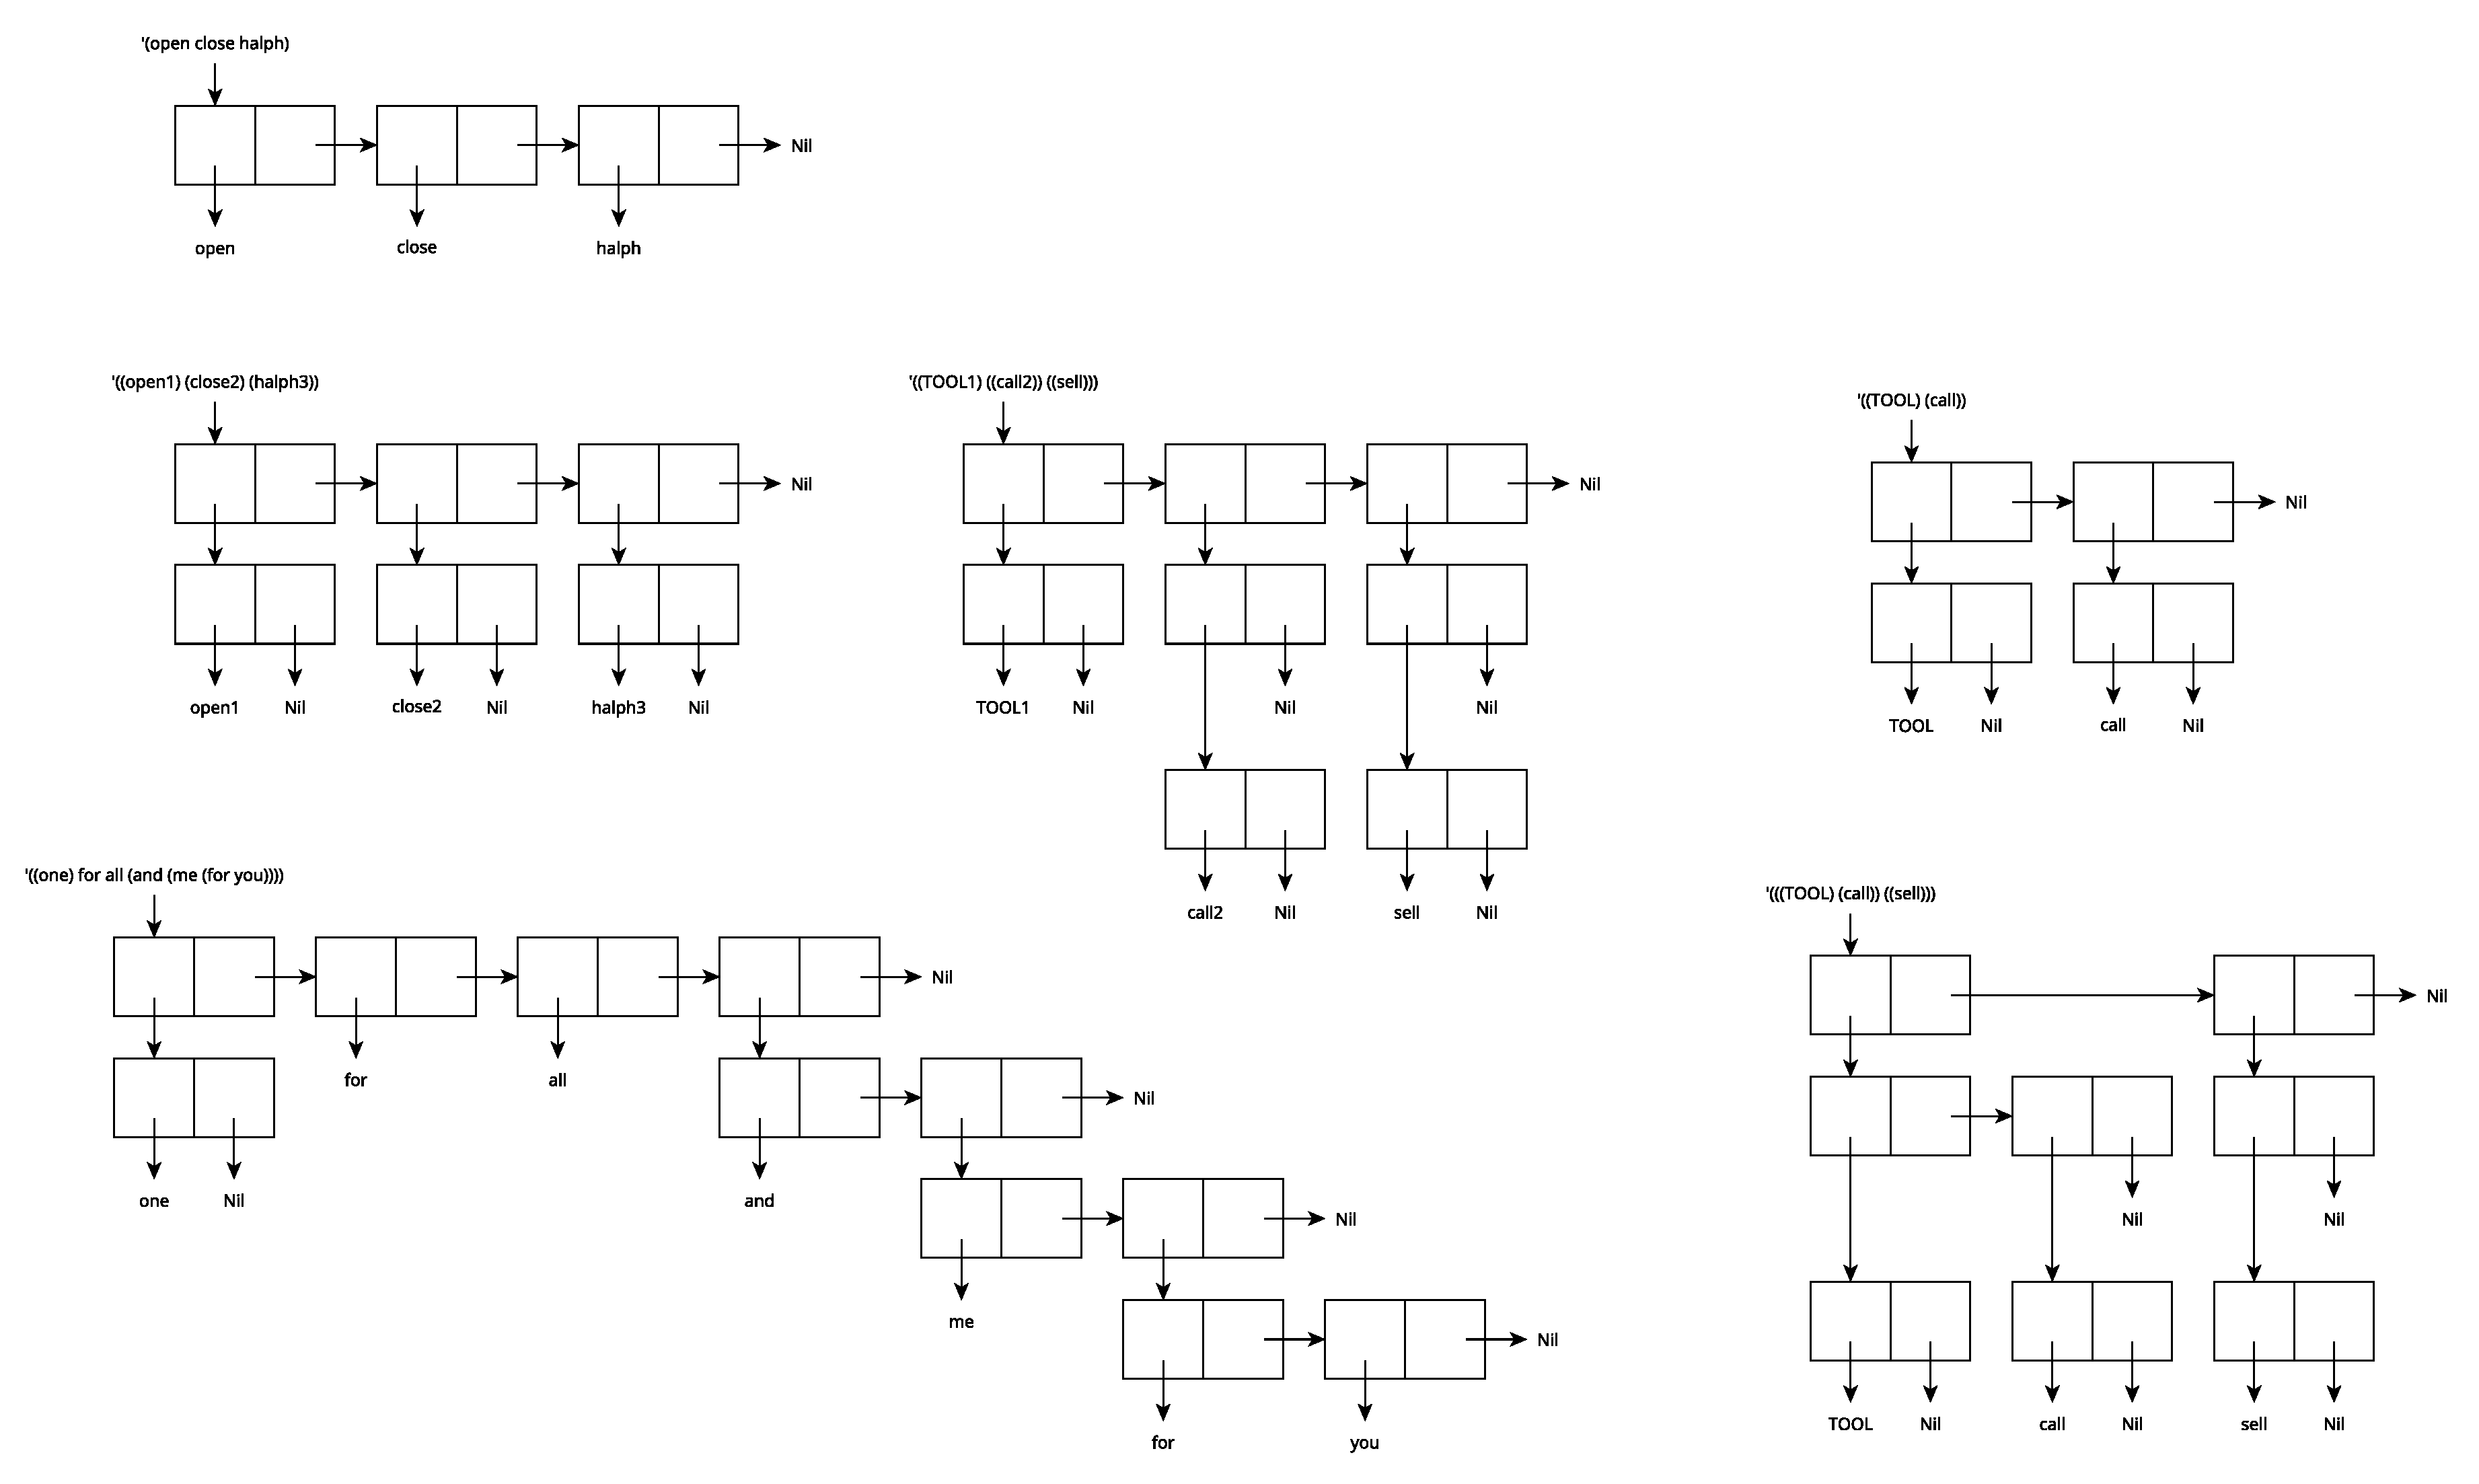
\includegraphics[width=0.8\linewidth]{1}
	\caption{Список '(open close halph)}
	\label{1_1}
\end{figure}
\begin{figure}[H]
	\centering
	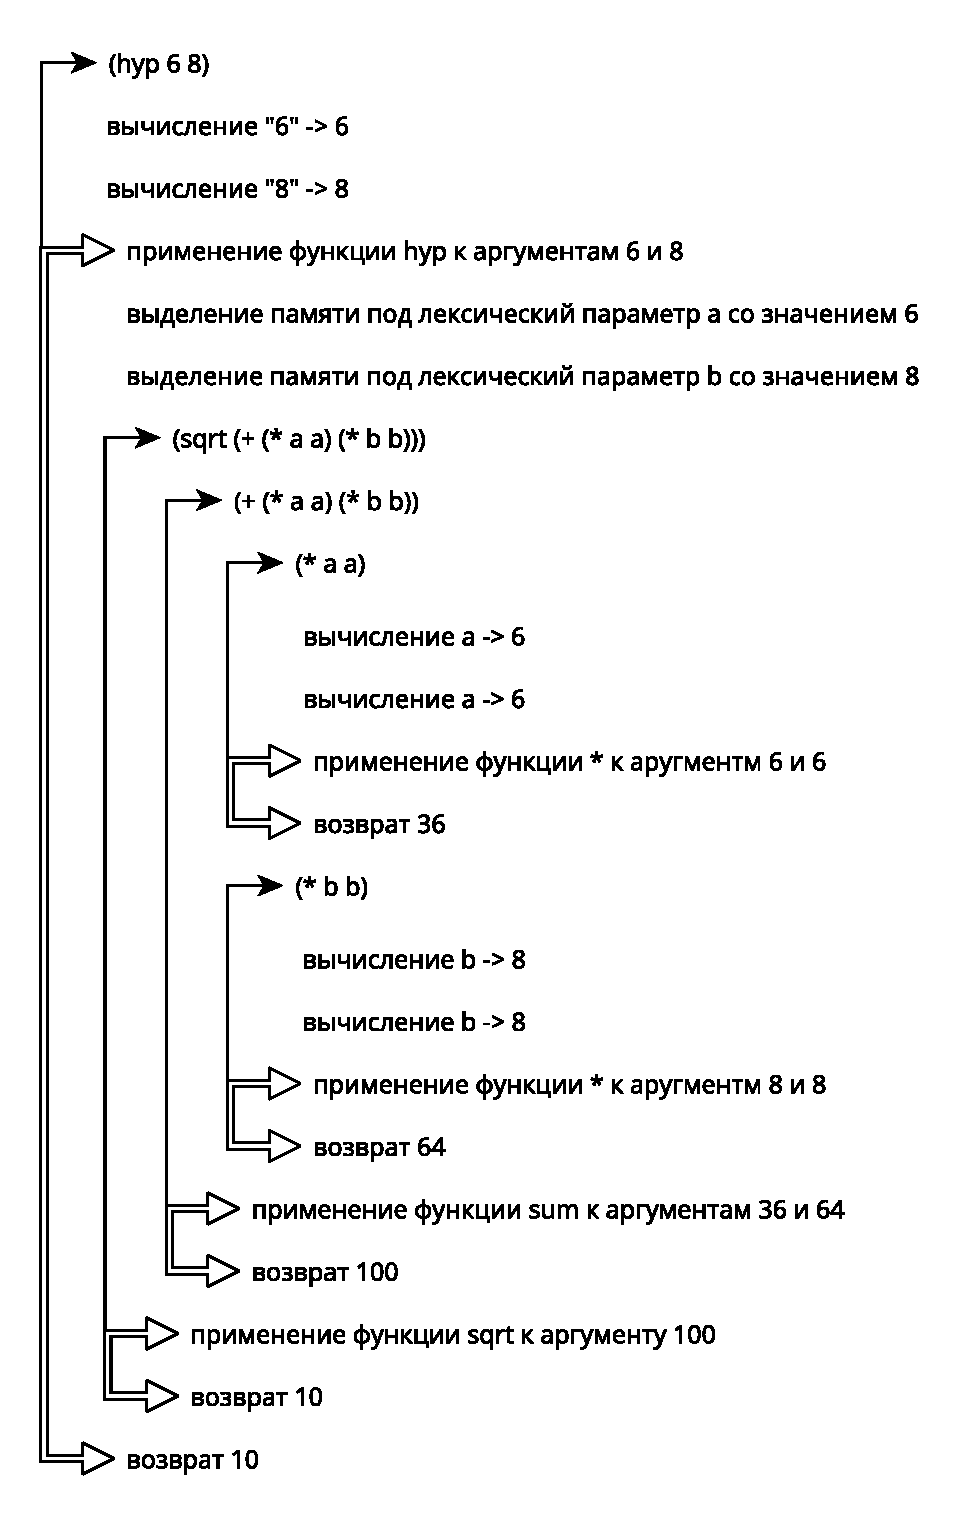
\includegraphics[width=0.8\linewidth]{2}
	\caption{Список '((open1) (close2) (halph3))}
	\label{1_2}
\end{figure}
\begin{figure}[H]
	\centering
	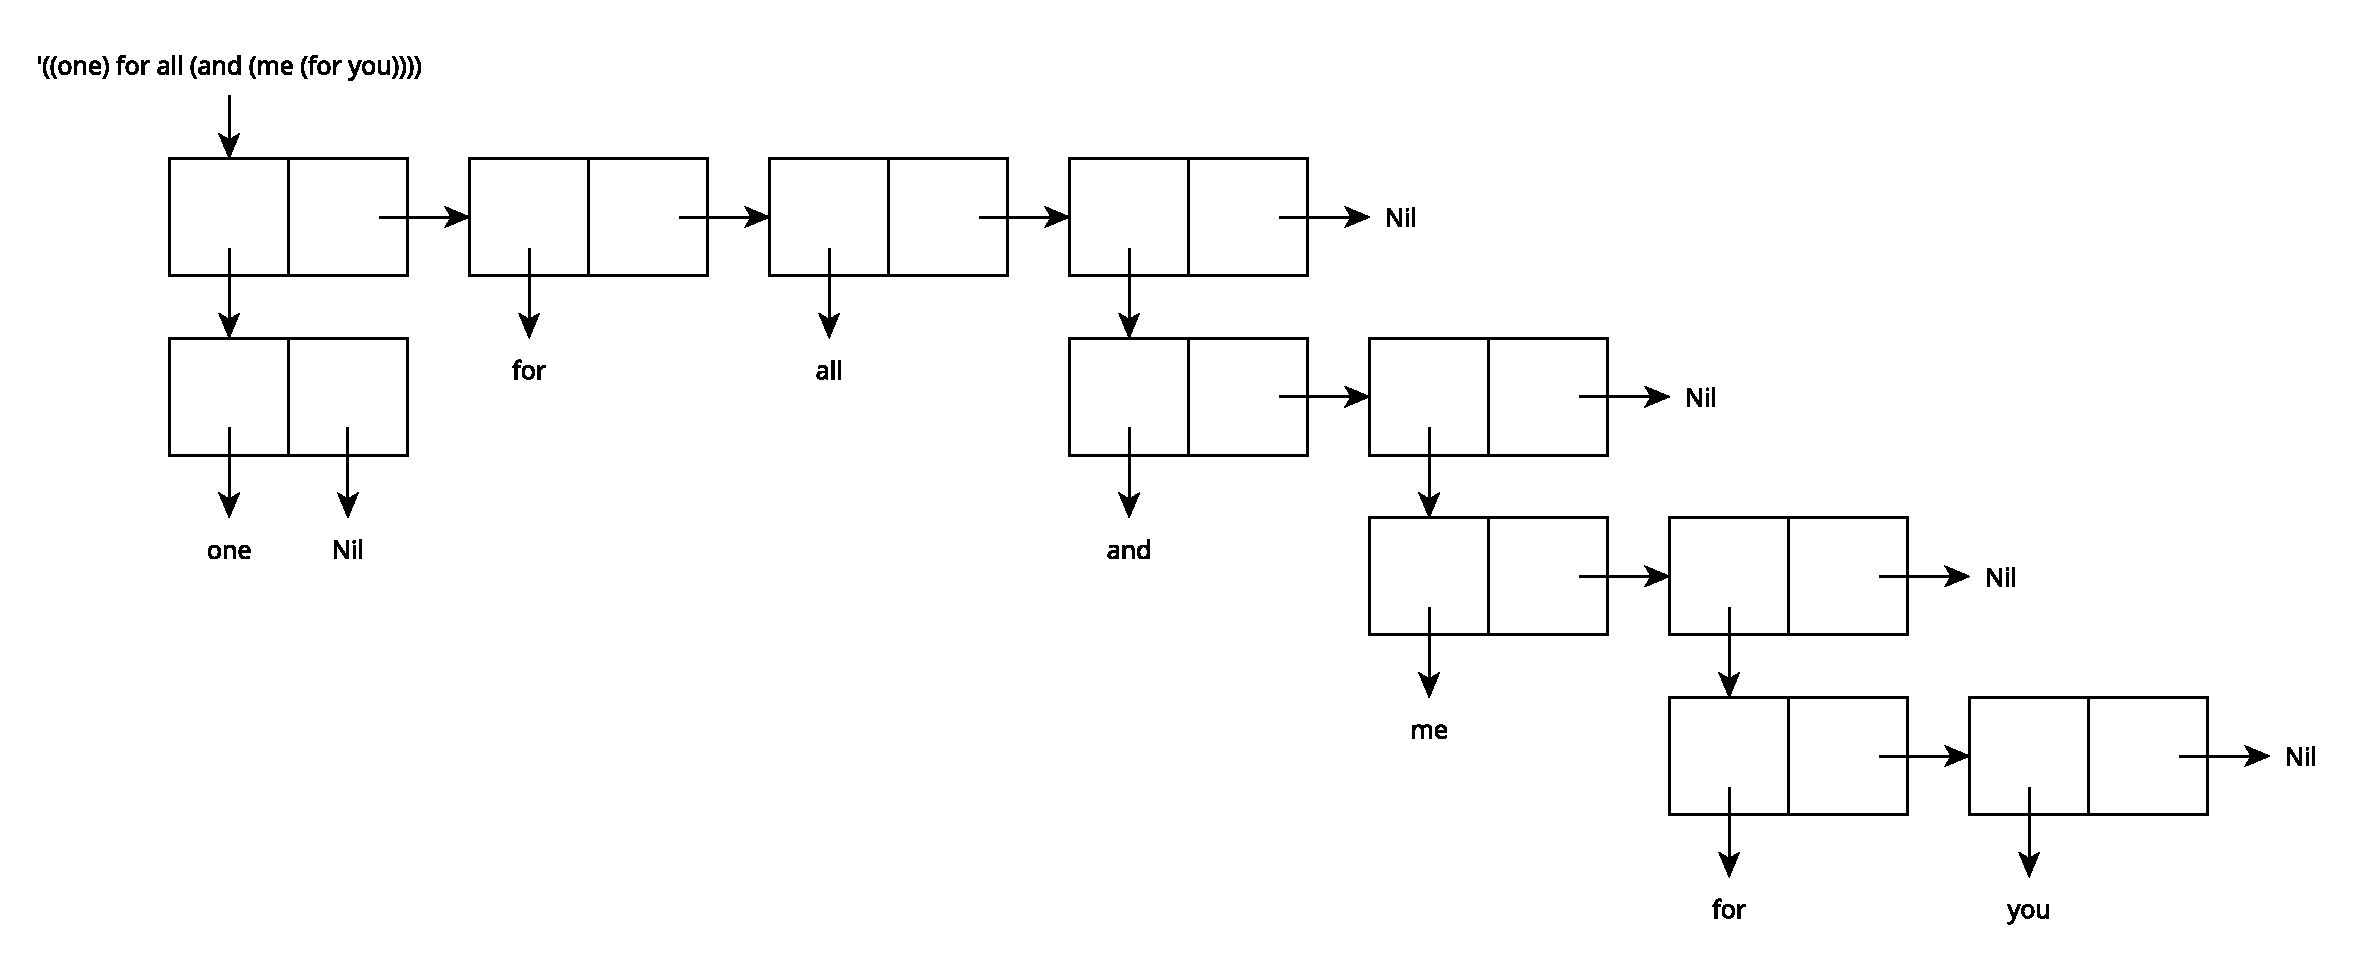
\includegraphics[width=\linewidth]{3}
	\caption{Список '((one) for all (and (me (for you)))) }
	\label{1_3}
\end{figure}
\begin{figure}[H]
	\centering
	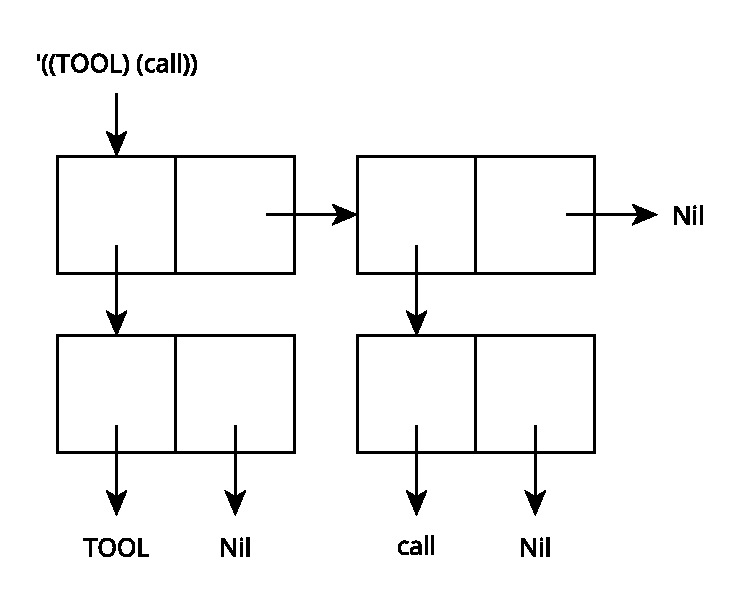
\includegraphics[width=0.6\linewidth]{4}
	\caption{Список '((TOOL) (call))}
	\label{1_4}
\end{figure}
\begin{figure}[H]
	\centering
	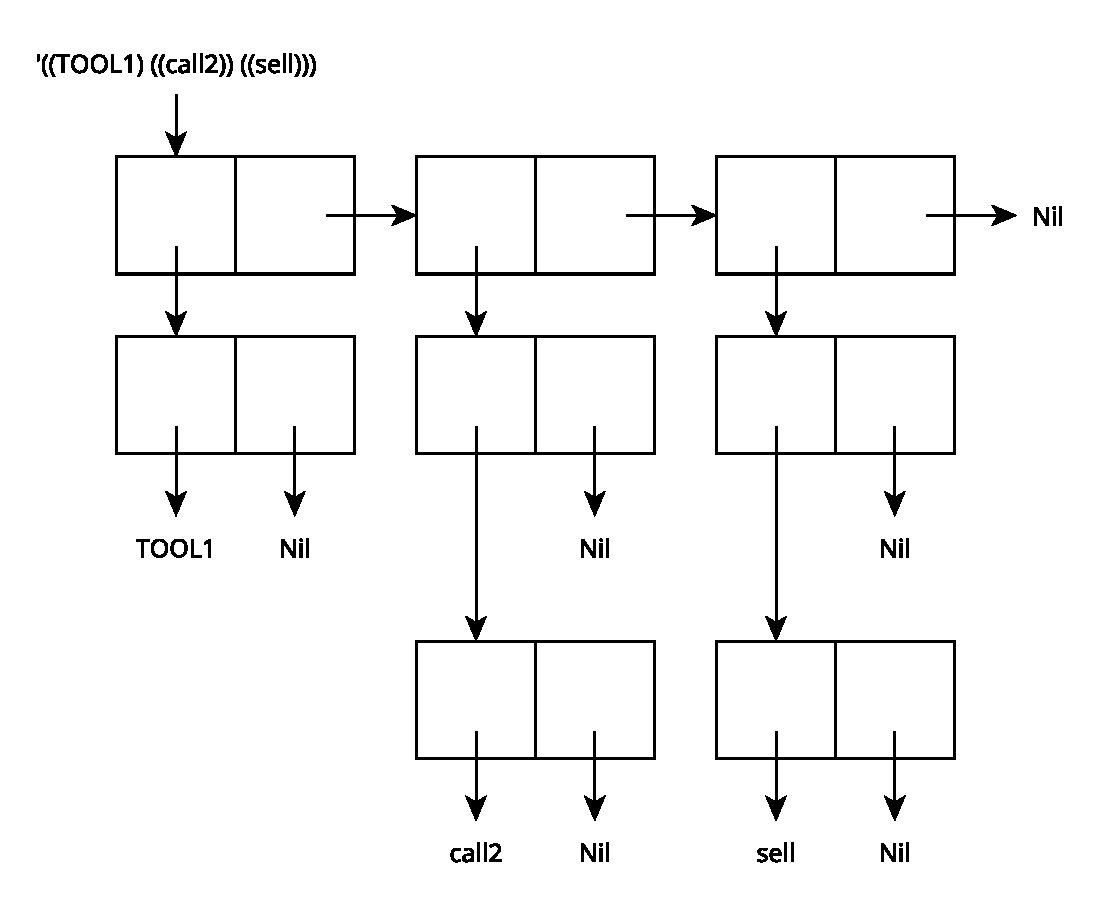
\includegraphics[width=0.6\linewidth]{5}
	\caption{Список '((TOOL1) ((call2)) ((sell)))}
	\label{1_5}
\end{figure}
\begin{figure}[H]
	\centering
	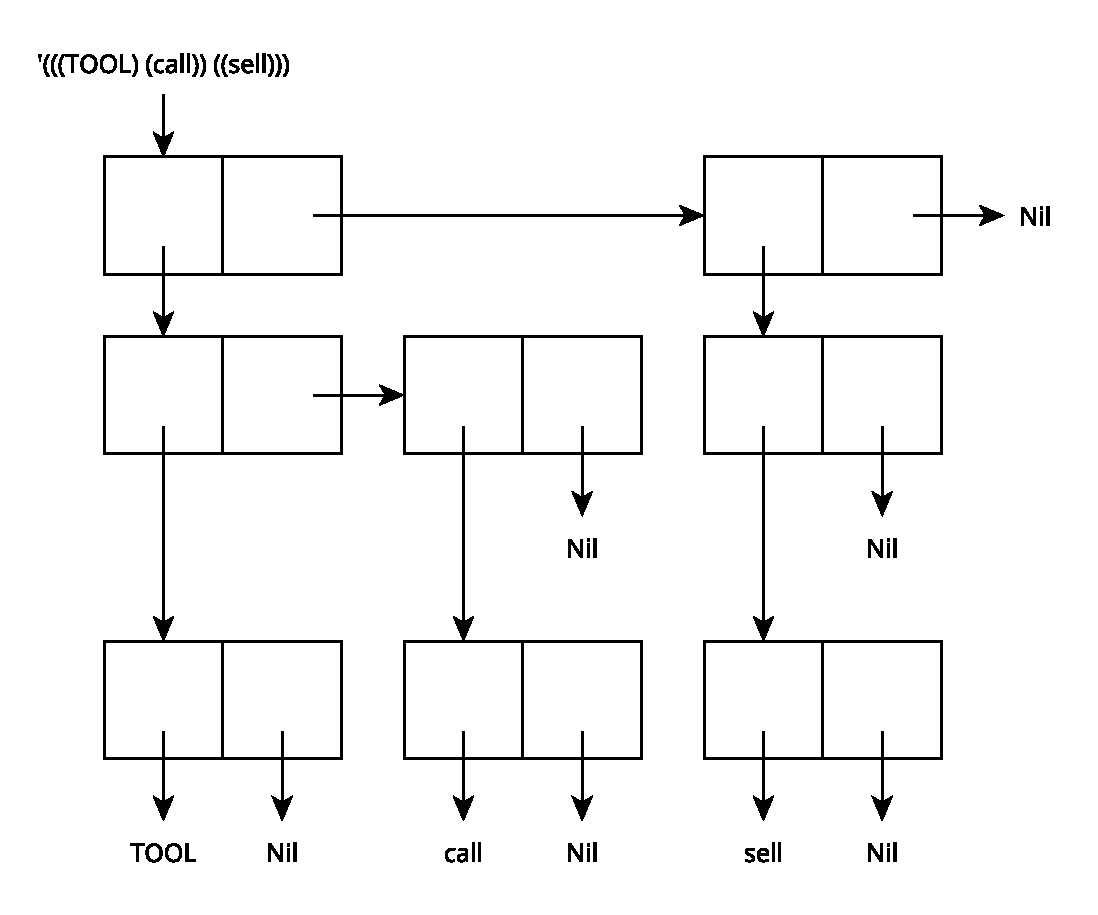
\includegraphics[width=0.8\linewidth]{6}
	\caption{Список '(((TOOL) (call)) ((sell)))}
	\label{1_6}
\end{figure}

\clearpage

\section{Задание 2}

\begin{lstlisting}
(car (cdr '(first second third fourth)))
(car (cdr (cdr '(first second third fourth))))
(car (cdr (cdr (cdr '(first second third fourth)))))
\end{lstlisting}

\section{Задание 3}

В таблице \ref{3} представлены результаты вычисления выражений.

\begin{center}
	\begin{threeparttable}
		\captionsetup{justification=raggedright,singlelinecheck=off}
		\caption{\label{3}Результаты вычисления выражений}
		\centering
		\begin{tabular}{|c|c|}
			\hline
			Выражение & Результат \\
			\hline
			(CAADR '((blue cube) (red pyramid))) & red \\
			\hline
			(CDAR '((abc) (def) (ghi))) & Nil \\
			\hline
			(CADR '((abc) (def) (ghi))) & (def) \\
			\hline
			(CADDR '((abc) (def) (ghi))) & (ghi) \\
			\hline
		\end{tabular}
	\end{threeparttable}
\end{center}

\section{Задание 4}

В таблице \ref{4} представлены результаты вычисления выражений.

\begin{center}
	\captionsetup{justification=raggedright,singlelinecheck=off}
	\begin{longtable}[c]{|c|c|c|}
		\caption{\label{4}Результаты вычисления выражений}\\
		\hline
		Выражение & Результат & Объяснение \\
		\hline
		(list 'Fred 'and 'Wilma) & (Fred and Wilma) & \specialcell{Создается список, состоящий\\из атомов Fred, and и Wilma,\\переданных функции list\\в качестве фактических\\параметров}\\
		\hline
		(cons 'Fred '(and Wilma)) & (Fred and Wilma) & \specialcell{Создается бинарный узел,\\первый указатель которого\\ссылается на атом Fred,\\а второй~--- на список (and Wilma).\\Так как второй указатель узла\\ссылается на список, то в\\результате получается список\\(Fred and Wilma)}\\
		\hline
		(list 'Fred '(and Wilma)) & (Fred (and Wilma)) & \specialcell{Создается список, состоящий\\из атома Fred и списка (and Wilma),\\переданных функции list\\в качестве фактических\\параметров}\\
		\hline
		(cons 'Fred '(Wilma)) & (Fred Wilma) & \specialcell{Создается бинарный узел,\\первый указатель которого\\ссылается на атом Fred,\\а второй~--- на список (Wilma).\\Так как второй указатель узла\\ссылается на список, то в\\результате получается список\\(Fred Wilma)}\\
		\hline
		(cons Nil Nil) & (Nil) & \specialcell{Создается бинарный узел,\\первый и второй указатели\\ которого ссылаются\\на пустые списки.\\Так как второй указатель узла\\ссылается на пустой список, то в\\результате получается список\\(Nil)}\\
		\hline
		(list Nil Nil) & (Nil Nil) & \specialcell{Создается список, состоящий\\из двух пустых списков,\\переданных функции list\\в качестве фактических\\параметров}\\
		\hline
		(cons T Nil) & (T) & \specialcell{Создается бинарный узел,\\первый указатель которого\\ссылается на атом T,\\а второй~--- на пустой список.\\Так как второй указатель узла\\ссылается на пустой список, то в\\результате получается список\\(T)}\\
		\hline
		(list T Nil) & (T Nil) & \specialcell{Создается список, состоящий\\из атома T и пустого списка,\\переданных функции cons в\\качестве фактических параметров}\\
		\hline
		(cons Nil T) & (Nil . T) & \specialcell{Создается бинарный узел,\\первый указатель которого\\ссылается на пустой список,\\а второй~--- на атом T}\\
		\hline
		(list Nil T) & (Nil T) & \specialcell{Создается список, состоящий\\из пустого списка\\и атома T, переданных\\функции list в качестве\\фактических параметров}\\
		\hline
		(list Nil) & (Nil) & \specialcell{Создается список, содержащий\\в себе пустой список,\\переданный функции list\\в качестве фактического\\параметра}\\
		\hline
		(cons T (list Nil)) & (T Nil) & \specialcell{Создается бинарный узел,\\первый указатель которого\\ссылается на атом T,\\а второй~--- на\\результат выполнения\\функции list. Так как\\результат выполнения (list Nil)\\является списком, содержащим\\в себе пустой список,\\то по итогу получается\\список (T Nil)}\\
		\hline
		(cons '(T) Nil) & ((T)) & \specialcell{Создается бинарный узел,\\первый указатель которого\\ссылается на список (T),\\а второй~--- на пустой список.\\Так как второй указатель узла\\ссылается на пустой список, то в\\результате получается список\\((T))}\\
		\hline
		(list '(T) Nil) & ((T) Nil) & \specialcell{Создается список, состоящий\\из списка (T) и\\пустого списка,\\переданных функции list\\в качестве фактических\\параметров}\\
		\hline
		(list '(one two) '(free temp)) & ((one two) (free temp)) & \specialcell{Создается список, состоящий\\из списков\\(one two) и (free temp)\\переданных функции list\\в качестве фактических\\параметров}\\
		\hline
		(cons '(one two) '(free temp)) & ((one two) free temp) & \specialcell{Создается бинарный узел,\\первый указатель которого\\ссылается на список (one two),\\а второй~--- на список (free temp).\\Так как второй указатель узла\\ссылается на список, то в\\результате получается список\\((one two) free temp)}\\
		\hline
	\end{longtable}
\end{center}

\clearpage

\section{Задание 5}

\begin{lstlisting}
; 1
(defun f1 (ar1 ar2 ar3 ar4) (list (list ar1 ar2) (list ar3 ar4)))
(lambda (ar1 ar2 ar3 ar4) (list (list ar1 ar2) (list ar3 ar4)))

; 2
(defun f2 (ar1  ar2) (list (list ar1) (list ar2)))
(lambda (ar1  ar2) (list (list ar1) (list ar2)))

; 3
(defun f3 (ar1) (list (list (list ar1))))
(lambda (ar1) (list (list (list ar1))))
\end{lstlisting}

На рисунках \ref{5_1}~--~\ref{5_3} представлены результаты функций в виде списочных ячеек.

\begin{figure}[H]
	\centering
	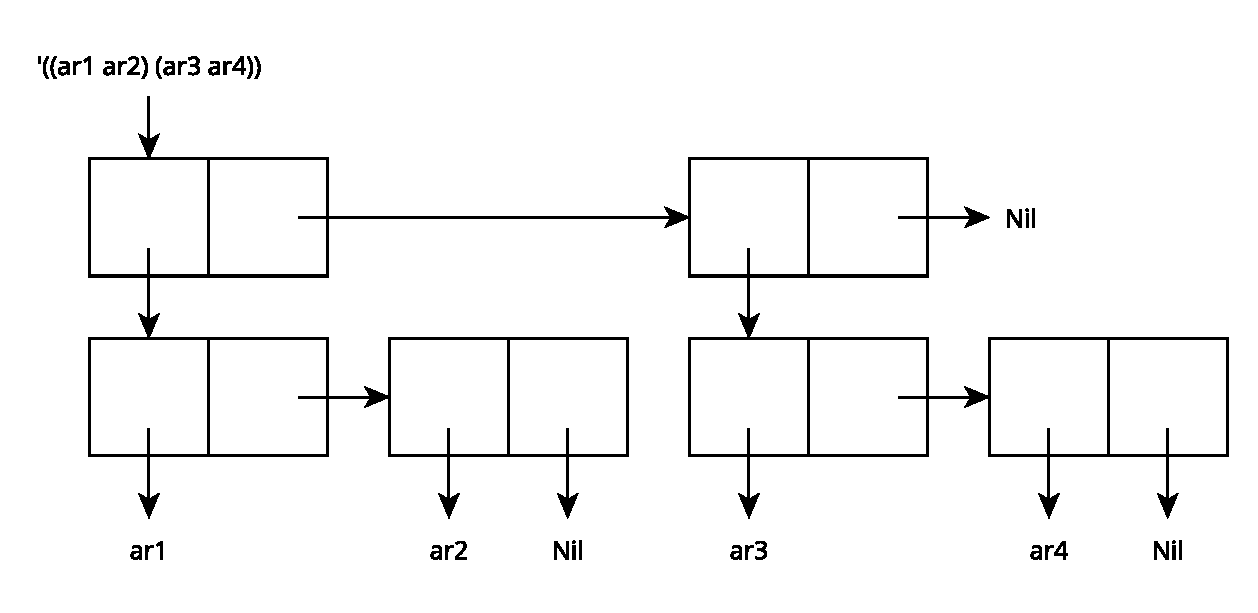
\includegraphics[width=0.8\linewidth]{5_1}
	\caption{Список '((ar1 ar2) (ar3 ar4))}
	\label{5_1}
\end{figure}
\begin{figure}[H]
	\centering
	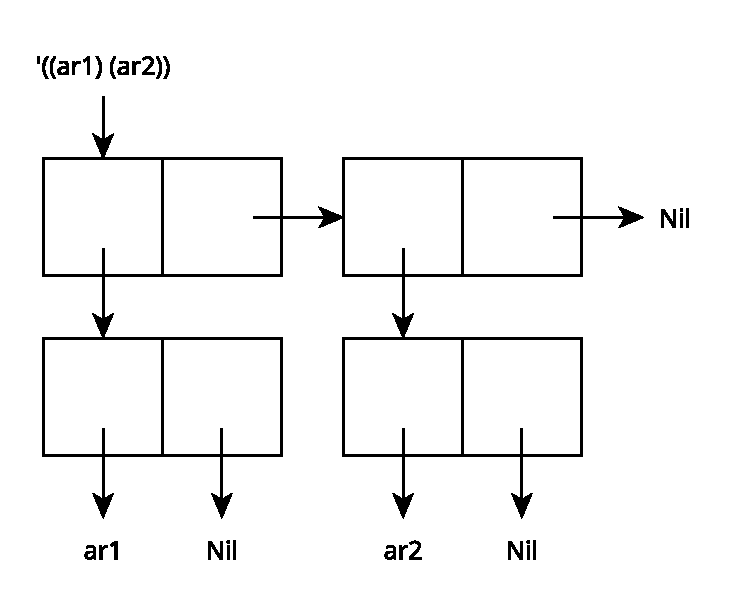
\includegraphics[width=0.55\linewidth]{5_2}
	\caption{Список '((ar1) (ar2))}
	\label{5_2}
\end{figure}
\begin{figure}[H]
	\centering
	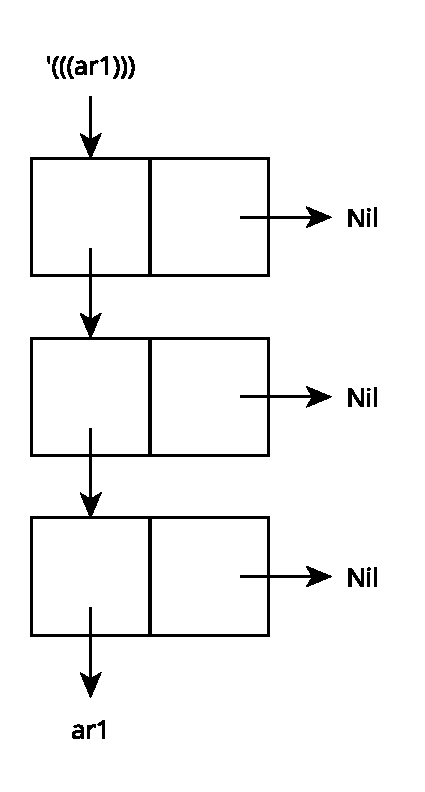
\includegraphics[width=0.3\linewidth]{5_3}
	\caption{Список '(((ar1)))}
	\label{5_3}
\end{figure}

\clearpage
